\documentclass[11pt]{article}

% ============================================================
%  Visual atlas of the patterns formalised in this library
%  Dempwolff--Mueller: permutation polynomials & translation
%  planes of even order.  Minimal words, many pictures.
% ============================================================

\usepackage[a4paper,margin=16mm]{geometry}
\usepackage{amsmath,amssymb}
\usepackage{tikz}
\usepackage{tikz-cd}
\usepackage{xcolor}
\usepackage{parskip}
\usetikzlibrary{arrows.meta,positioning,calc,decorations.pathmorphing,
  decorations.markings,shapes.geometric,shapes.misc,backgrounds,fit,
  graphs,quotes,patterns,matrix,chains,angles}

% ---- palette -------------------------------------------------
\definecolor{cA}{HTML}{1b4965}
\definecolor{cB}{HTML}{5fa8d3}
\definecolor{cC}{HTML}{cae9ff}
\definecolor{cD}{HTML}{e07a5f}
\definecolor{cE}{HTML}{81b29a}
\definecolor{cF}{HTML}{f2cc8f}
\definecolor{cG}{HTML}{6a4c93}
\definecolor{ink}{HTML}{22223b}

% ---- reusable styles -----------------------------------------
\tikzset{
  dot/.style={circle,fill=cA,inner sep=1.6pt},
  odot/.style={circle,draw=cA,fill=white,inner sep=1.6pt},
  box/.style={rounded corners=2pt,draw=cA,thick,fill=cC,
              inner sep=4pt,align=center},
  chip/.style={rounded corners=3pt,draw=cA,very thick,fill=cF,
              inner sep=5pt,align=center,font=\small},
  maparrow/.style={-{Stealth[length=3mm]},thick,cA},
  bij/.style={<->,{Stealth[length=2.6mm]}-{Stealth[length=2.6mm]},thick,cD},
  wavy/.style={decorate,decoration={snake,amplitude=.6mm,segment length=2mm}},
}

\newcommand{\GF}[1]{\mathrm{GF}(#1)}
\newcommand{\Tr}{\mathrm{T}}
\newcommand{\heading}[2]{%
  \begin{center}\begin{tikzpicture}
    \node[fill=cA,text=white,rounded corners=3pt,inner xsep=8pt,inner ysep=4pt,
      font=\large\bfseries] (h){#1};
  \end{tikzpicture}\end{center}
  \begin{center}\itshape\small #2\end{center}\vspace{-2mm}}

\pagestyle{empty}

\begin{document}

% =============================================================
% TITLE
% =============================================================
\begin{center}

\begin{tikzpicture}
  \node[font=\Huge\bfseries,text=cA] {Pictures of the Patterns};
\end{tikzpicture}\\[2mm]
{\large Permutation polynomials \& translation planes of even order}\\[1mm]
{\small a visual atlas of everything the Lean library proves --- few words, many diagrams}
\end{center}

\vspace{2mm}

% ---- One field, one map: the master idea ----
\begin{center}
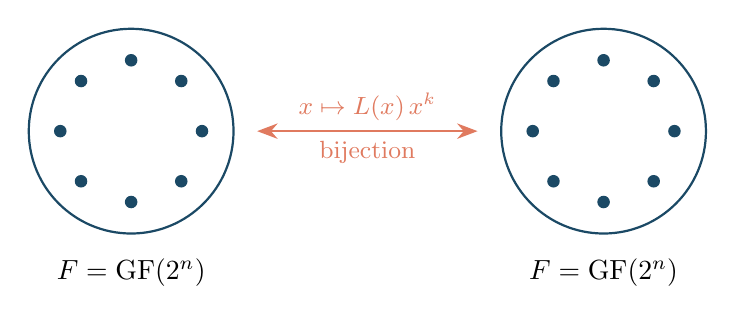
\begin{tikzpicture}[scale=1]
  % field on left
  \foreach \a in {0,45,...,315}{
     \node[dot] (L\a) at ({0.9*cos(\a)},{0.9*cos(\a)*0+0.9*sin(\a)}) {};
  }
  \node[draw=cA,thick,circle,minimum size=2.6cm] (Fl) at (0,0){};
  \node[below=1.5cm] at (0,0) {$F=\GF{2^n}$};
  % field on right
  \begin{scope}[xshift=6cm]
    \foreach \a in {0,45,...,315}{
       \node[dot] (R\a) at ({0.9*cos(\a)},{0.9*sin(\a)}) {};
    }
    \node[draw=cA,thick,circle,minimum size=2.6cm] at (0,0){};
    \node[below=1.5cm] at (0,0) {$F=\GF{2^n}$};
  \end{scope}
  % arrow
  \draw[bij] (1.6,0) -- (4.4,0) node[midway,above,font=\small]{$x\mapsto L(x)\,x^{k}$}
     node[midway,below,font=\small,cD]{bijection};
\end{tikzpicture}
\end{center}

\begin{center}\small
Everything below lives on one finite field of even order.\\
The recurring shape: a map that permutes the whole field.
\end{center}

\vfill

% ---- library map (dependency quiver) ----
\heading{The library at a glance}{boxes = theories, arrows = ``builds on''}

\begin{center}
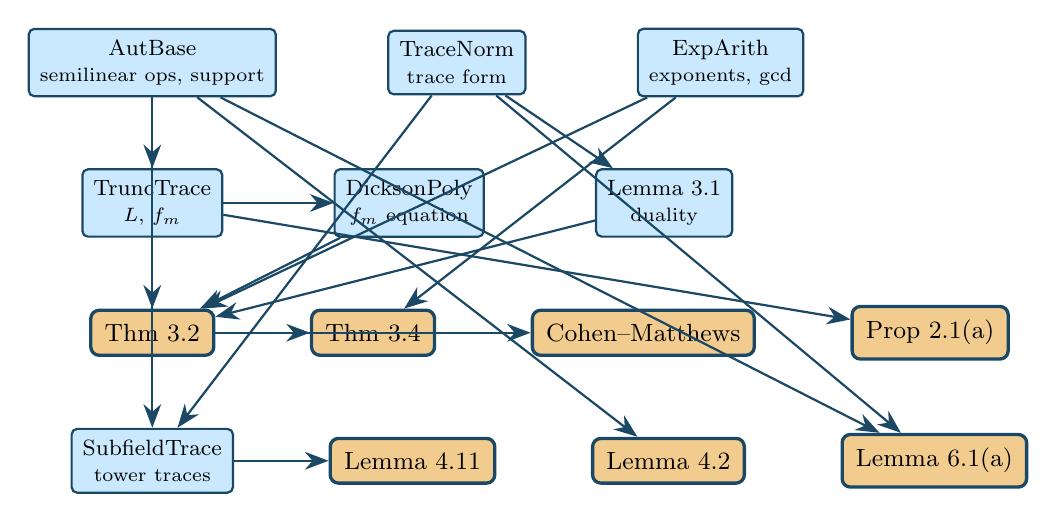
\begin{tikzpicture}[node distance=7mm,every node/.style={font=\footnotesize}]
  \node[box] (auto) {AutBase\\\scriptsize semilinear ops, support};
  \node[box,right=14mm of auto] (tr) {TraceNorm\\\scriptsize trace form};
  \node[box,right=14mm of tr] (exp) {ExpArith\\\scriptsize exponents, gcd};

  \node[box,below=9mm of auto] (tt) {TruncTrace\\\scriptsize $L$, $f_m$};
  \node[box,right=14mm of tt] (dick) {DicksonPoly\\\scriptsize $f_m$ equation};
  \node[box,right=14mm of dick] (l31) {Lemma 3.1\\\scriptsize duality};

  \node[chip,below=9mm of tt] (t32) {Thm 3.2};
  \node[chip,right=12mm of t32] (t34) {Thm 3.4};
  \node[chip,right=12mm of t34] (cm) {Cohen--Matthews};
  \node[chip,right=12mm of cm] (qf) {Prop 2.1(a)};

  \node[box,below=9mm of t32] (sub) {SubfieldTrace\\\scriptsize tower traces};
  \node[chip,right=12mm of sub] (l411) {Lemma 4.11};
  \node[chip,right=12mm of l411] (l42) {Lemma 4.2};
  \node[chip,right=12mm of l42] (l61) {Lemma 6.1(a)};

  \graph[use existing nodes,edges={maparrow}]{
    auto->tt; auto->l42; auto->l61;
    tr->l31; tr->l61; tr->sub;
    exp->t32; exp->t34;
    tt->{dick,t32}; dick->t32; l31->t32;
    t32->{t34,cm}; tt->qf;
    sub->{l411}; auto->sub;
  };
\end{tikzpicture}
\end{center}

\newpage
% =============================================================
% 1. Permutation polynomial
% =============================================================
\heading{1. The core object: a permutation polynomial}{$P(x)=L(x)\cdot x^{k}$ shuffles $F$ with no clashes and no gaps}

\begin{center}
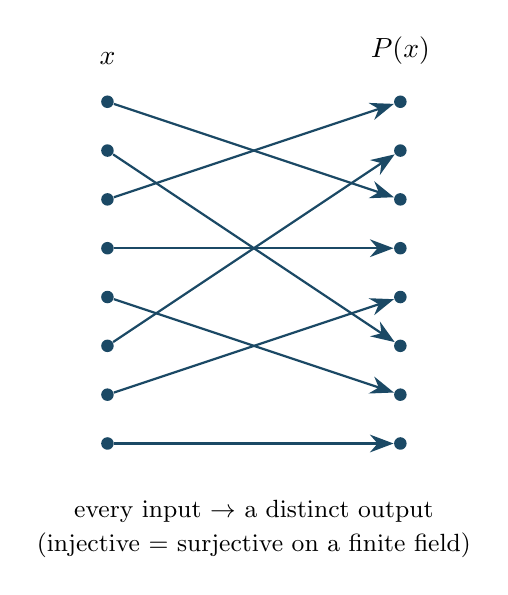
\begin{tikzpicture}[scale=.62]
  % vertical dots two columns, a permutation
  \foreach \i/\j in {0/2,1/5,2/0,3/3,4/6,5/1,6/4,7/7}{
     \node[dot] (a\i) at (0,-\i){};
     \node[dot] (b\i) at (6,-\i){};
  }
  \foreach \i/\j in {0/2,1/5,2/0,3/3,4/6,5/1,6/4,7/7}{
     \draw[maparrow] (a\i) -- (b\j);
  }
  \node[above=1mm] at (0,.4) {$x$};
  \node[above=1mm] at (6,.4) {$P(x)$};
  \node[below=6mm,align=center] at (3,-7) {\small every input $\to$ a distinct output\\\small (injective $=$ surjective on a finite field)};
\end{tikzpicture}
\qquad
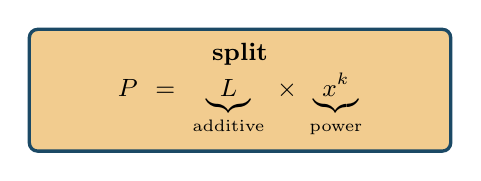
\begin{tikzpicture}[baseline=(c.base)]
  \node[chip,text width=5cm] (c) {\textbf{split}\\[2pt]
   $P = \underbrace{L}_{\text{additive}}\ \times\ \underbrace{x^{k}}_{\text{power}}$};
\end{tikzpicture}
\end{center}

\vspace{2mm}
\heading{additive part $L$: a straight line through $0$}{$L(a+b)=L(a)+L(b)$; if $P$ is a bijection then so is $L$}

\begin{center}
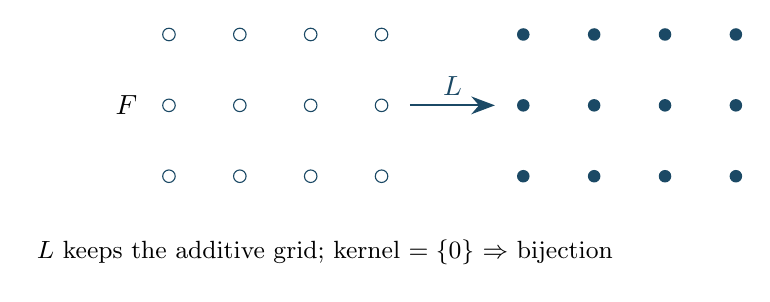
\begin{tikzpicture}[scale=.9]
  % grid lattice of F_2 vector space, L linear
  \foreach \x in {0,...,3}\foreach \y in {0,...,2}{
     \node[odot] at (\x,\y){};}
  \node at (-.6,1) {$F$};
  \draw[maparrow] (3.4,1)--(4.6,1) node[midway,above]{$L$};
  \begin{scope}[xshift=5cm]
  \foreach \x in {0,...,3}\foreach \y in {0,...,2}{
     \node[dot] at (\x,\y){};}
  \end{scope}
  \node[below=5mm,align=center] at (2.2,-.2)
    {\small $L$ keeps the additive grid; kernel $=\{0\}$ $\Rightarrow$ bijection};
\end{tikzpicture}
\end{center}

\vspace{3mm}
\heading{power part $x^{k}$: winding the unit circle}{on $F^\ast$ it is $\times k$ on the cyclic group $\mathbb Z/(2^n-1)$}

\begin{center}
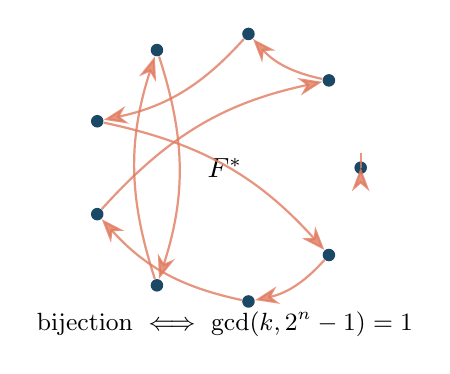
\begin{tikzpicture}[scale=1.15]
  \def\N{9}
  \foreach \i in {1,...,\N}{
    \node[dot] (u\i) at ({360/\N*\i}:1.5){};
  }
  \node at (0,0) {$F^\ast$};
  % map x->x^2 (k=2) arrows
  \foreach \i in {1,...,\N}{
    \pgfmathtruncatemacro\j{Mod(2*\i,\N)==0 ? \N : Mod(2*\i,\N)}
    \draw[maparrow,cD,opacity=.8] (u\i) to[bend left=18] (u\j);
  }
  \node[below=1.7cm] at (0,0){\small bijection $\iff$ $\gcd(k,2^n-1)=1$};
\end{tikzpicture}
\end{center}

\newpage
% =============================================================
% 2. Lemma 3.1 duality / adjoint iso
% =============================================================
\heading{2. Lemma 3.1 --- a duality (iso-equivalence)}{$L(x)M(x)$ injective $\iff$ $L^\ast(x)M^{-1}(x)$ injective}

\begin{center}
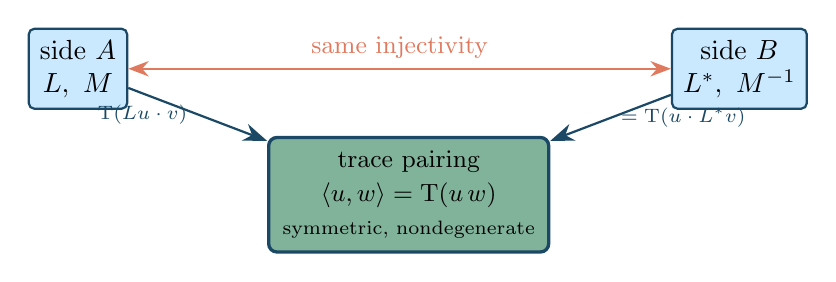
\begin{tikzpicture}[scale=1]
  % the trace pairing in the middle
  \node[chip,fill=cE] (pair) at (0,0) {trace pairing\\[1pt]$\langle u,w\rangle=\Tr(u\,w)$\\[1pt]\scriptsize symmetric, nondegenerate};
  \node[box] (L) at (-4.2,1.6) {side $A$\\$L,\ M$};
  \node[box] (Ls) at (4.2,1.6) {side $B$\\$L^\ast,\ M^{-1}$};
  \draw[bij] (L) -- (Ls) node[midway,above,font=\small]{same injectivity};
  \draw[maparrow] (L) -- (pair) node[midway,left,font=\scriptsize]{$\Tr(Lu\cdot v)$};
  \draw[maparrow] (Ls) -- (pair) node[midway,right,font=\scriptsize]{$=\Tr(u\cdot L^\ast v)$};
\end{tikzpicture}
\end{center}

\vspace{2mm}
\heading{the adjoint square commutes}{$L$ bijective $\iff$ $L^\ast$ bijective under the pairing}

\begin{center}
\begin{tikzcd}[column sep=large,row sep=large]
F \arrow[r,"L"] \arrow[d,"{\langle\,\cdot\,,\,\cdot\,\rangle}"'] & F \arrow[d,"{\langle\,\cdot\,,\,\cdot\,\rangle}"] \\
F^{\vee} & F^{\vee} \arrow[l,"L^{\ast}"]
\end{tikzcd}
\qquad
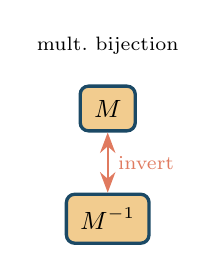
\begin{tikzpicture}[baseline]
  \node[chip] (M) at (0,0.7) {$M$};
  \node[chip] (Mi) at (0,-0.7) {$M^{-1}$};
  \draw[bij] (M)--(Mi) node[midway,right,font=\scriptsize]{invert};
  \node[font=\scriptsize] at (0,1.5){mult.\ bijection};
\end{tikzpicture}
\end{center}

\vspace{2mm}
\heading{the pairing turns products into a shift}{$\Delta_y(x)=L(xy)M(y)$; the two ``$\Delta$-planes'' are dual}

\begin{center}
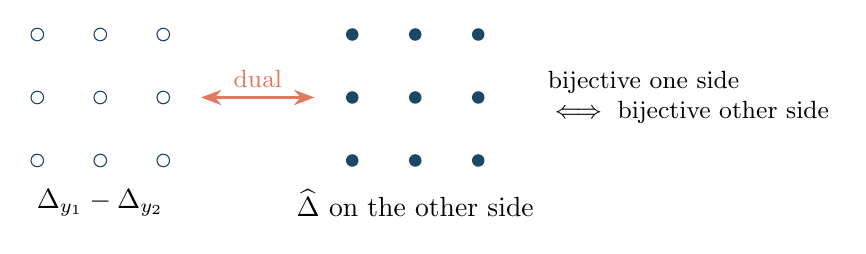
\begin{tikzpicture}[scale=.8]
  % two grids linked by trace form, showing self-duality
  \foreach \x in {0,1,2}\foreach \y in {0,1,2}{\node[odot] at (\x,\y){};}
  \node[below] at (1,-.3){$\Delta_{y_1}-\Delta_{y_2}$};
  \draw[bij] (2.6,1)--(4.4,1) node[midway,above,font=\small]{dual};
  \begin{scope}[xshift=5cm]
   \foreach \x in {0,1,2}\foreach \y in {0,1,2}{\node[dot] at (\x,\y){};}
   \node[below] at (1,-.3){$\widehat\Delta$ on the other side};
  \end{scope}
  \node[right=6mm,align=left,font=\small] at (7.2,1)
    {bijective one side\\$\iff$ bijective other side};
\end{tikzpicture}
\end{center}

\newpage
% =============================================================
% 3. Prop 2.1(a) quasifield
% =============================================================
\heading{3. Prop 2.1(a) --- a new multiplication}{$x\ast y=L(xy)\,x^{k}$ makes $F$ a weak quasifield}

\begin{center}
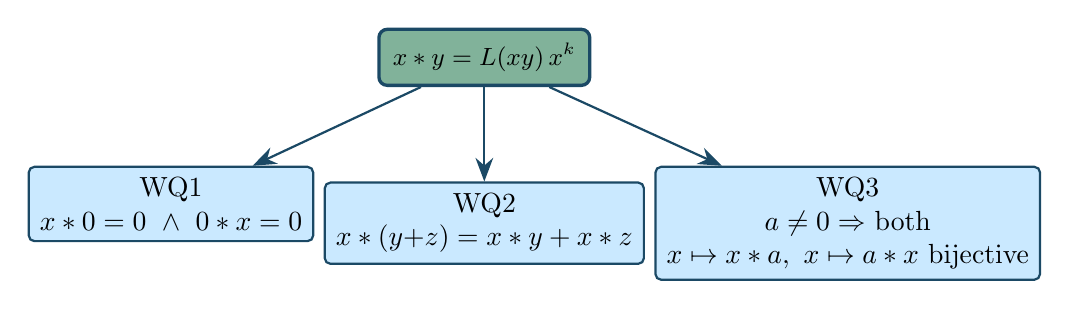
\begin{tikzpicture}[node distance=5mm]
  \node[chip,fill=cE] (m) {$x\ast y=L(xy)\,x^{k}$};
  \node[box,below left=10mm and 8mm of m] (w1) {WQ1\\$x\ast0=0\ \wedge\ 0\ast x=0$};
  \node[box,below=12mm of m] (w2) {WQ2\\$x\ast(y{+}z)=x\ast y+x\ast z$};
  \node[box,below right=10mm and 8mm of m] (w3) {WQ3\\$a\neq0\Rightarrow$ both\\$x\mapsto x\ast a,\ x\mapsto a\ast x$ bijective};
  \draw[maparrow](m)--(w1);\draw[maparrow](m)--(w2);\draw[maparrow](m)--(w3);
\end{tikzpicture}
\end{center}

\vspace{1mm}
\heading{WQ2 = left line stays a line}{multiplication by a fixed $x$ is additive}

\begin{center}
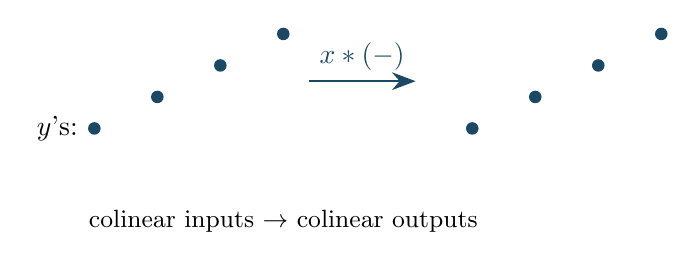
\begin{tikzpicture}[scale=.8]
  \foreach \i in {0,1,2,3}{\node[dot](p\i) at (\i,{0.5*\i}){};}
  \node[left] at (p0.west){$y$'s:};
  \draw[maparrow] (3.4,.75)--(5.1,.75) node[midway,above]{$x\ast(-)$};
  \begin{scope}[xshift=6cm]
   \foreach \i in {0,1,2,3}{\node[dot](q\i) at (\i,{0.5*\i}){};}
  \end{scope}
  \node[below=6mm] at (3,-.4){\small colinear inputs $\to$ colinear outputs};
\end{tikzpicture}
\end{center}

\vspace{1mm}
\heading{WQ3 = Latin square}{each nonzero row / column is a permutation}

\begin{center}
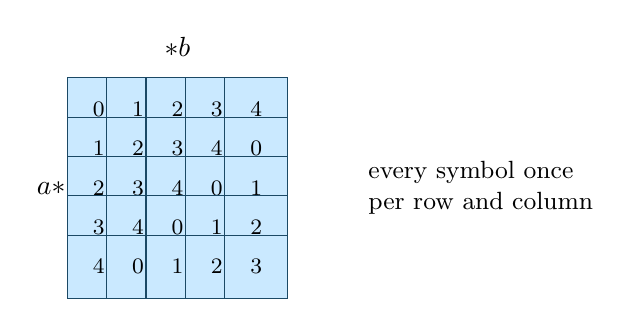
\begin{tikzpicture}[scale=.5]
  \foreach \r in {0,...,4}\foreach \c in {0,...,4}{
    \pgfmathtruncatemacro\v{Mod(\r+\c,5)}
    \definecolor{cell}{HTML}{cae9ff}
    \node[draw=cA,fill=cell,minimum size=8mm,inner sep=0] at (\c,-\r) {\footnotesize\v};
  }
  \node[left=3mm] at (0,-2){$a\ast$};
  \node[above=3mm] at (2,.5){$\ast b$};
  \node[right=8mm,align=left,font=\small] at (5,-2)
    {every symbol once\\per row and column};
\end{tikzpicture}
\end{center}

\newpage
% =============================================================
% 4. Theorem 3.2 (the concrete construction)
% =============================================================
\heading{4. Theorem 3.2 --- an explicit family}{on $\GF{2^n}$ with the right exponent, $L(x)x^{k}$ is a permutation}

\begin{center}
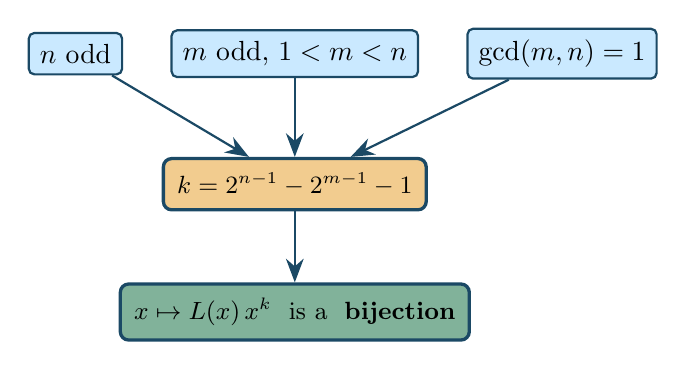
\begin{tikzpicture}[node distance=4mm]
  \node[box] (n) {$n$ odd};
  \node[box,right=6mm of n] (m) {$m$ odd,\ $1<m<n$};
  \node[box,right=6mm of m] (g) {$\gcd(m,n)=1$};
  \node[chip,fill=cF,below=10mm of m] (k)
     {$k=2^{n-1}-2^{m-1}-1$};
  \node[chip,fill=cE,below=9mm of k] (res)
     {$x\mapsto L(x)\,x^{k}$ \ is a \ \textbf{bijection}};
  \draw[maparrow](n)--(k);\draw[maparrow](m)--(k);\draw[maparrow](g)--(k);
  \draw[maparrow](k)--(res);
\end{tikzpicture}
\end{center}

\vspace{1mm}
\heading{how it is built: three ingredients meet}{truncated trace $L$, Dickson $f_m$, trace duality}

\begin{center}
\begin{tikzcd}[column sep=huge,row sep=large]
L(x)=\textstyle\sum_{i<m}x^{2^{i}}
   \arrow[dr,"\text{feeds}"'] & &
f_m \ (\text{Dickson})\arrow[dl,"\text{reduces}"]\\
 & \fbox{$L(x)\,x^{k}$ bijective} & \\
 & \text{Lemma 3.1 duality}\arrow[u,"\text{transfers}"'] &
\end{tikzcd}
\end{center}

\vspace{1mm}
\heading{Dickson functional equation}{$f_m$ separates $y$ from $y^{-1}$ on the units}

\begin{center}
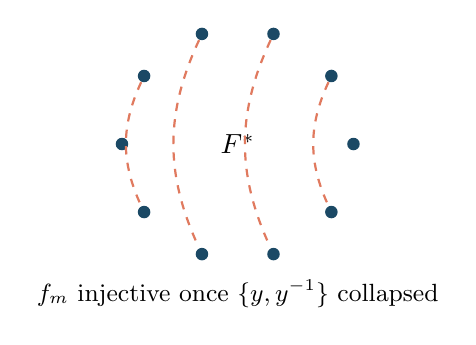
\begin{tikzpicture}[scale=1.05]
  \def\N{10}
  \foreach \i in {1,...,\N}{\node[dot](d\i) at ({360/\N*\i}:1.4){};}
  \node at (0,0){$F^\ast$};
  % pairs y <-> y^{-1}
  \foreach \i/\j in {1/9,2/8,3/7,4/6}{
     \draw[cD,thick,dashed] (d\i) to[bend right=25] (d\j);}
  \node[below=1.6cm] at (0,0){\small $f_m$ injective once $\{y,y^{-1}\}$ collapsed};
\end{tikzpicture}
\end{center}

\newpage
% =============================================================
% 5. Theorem 3.4 : functorial transfer
% =============================================================
\heading{5. Theorem 3.4 --- functorial transfer}{one permutation gives a whole family, via a commuting triangle}

\begin{center}
\begin{tikzcd}[column sep=huge,row sep=large]
F \arrow[rr,"x\,\mapsto\,L(x)\,x^{k+b}"] \arrow[dr,"z\,\mapsto\,z^{1+b\ell}"'{yshift=-1mm}] & & F\\
 & F \arrow[ur,"x\,\mapsto\,L(x)\,x^{k}"'{yshift=-1mm}] &
\end{tikzcd}
\end{center}

\begin{center}\small
new map $=$ (old permutation) $\circ$ (a power permutation)\ \ $\Rightarrow$\ \ still a bijection.
\end{center}

\vspace{2mm}
\heading{side conditions = gcd gates}{the two factors are bijections exactly when their gcd's vanish}

\begin{center}
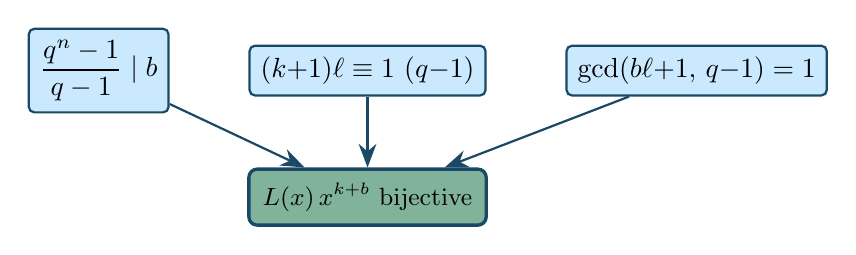
\begin{tikzpicture}[node distance=6mm]
  \node[box] (a){$\dfrac{q^{n}-1}{q-1}\mid b$};
  \node[box,right=10mm of a] (b){$(k{+}1)\ell\equiv1\ (q{-}1)$};
  \node[box,right=10mm of b] (c){$\gcd(b\ell{+}1,\,q{-}1)=1$};
  \node[chip,fill=cE,below=9mm of b] (r){$L(x)\,x^{k+b}$ bijective};
  \draw[maparrow](a)--(r);\draw[maparrow](b)--(r);\draw[maparrow](c)--(r);
\end{tikzpicture}
\end{center}

\vspace{2mm}
\heading{the family, pictured}{shifting $k$ by multiples of $b$ keeps the bijection}

\begin{center}
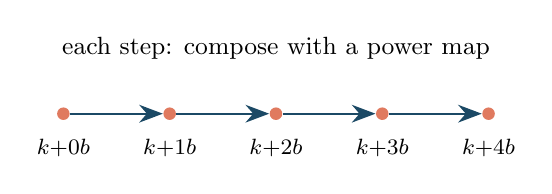
\begin{tikzpicture}[scale=.9]
  \foreach \i in {0,...,4}{
     \node[dot,fill=cD] (e\i) at (\i*1.5,0){};
     \node[below=2mm] at (e\i){\footnotesize $k{+}\i b$};
  }
  \foreach \i in {0,...,3}{
     \pgfmathtruncatemacro\j{\i+1}
     \draw[maparrow] (e\i)--(e\j);
  }
  \node[above=3mm] at (3,.3){\small each step: compose with a power map};
\end{tikzpicture}
\end{center}

\newpage
% =============================================================
% 6. Cohen--Matthews connection
% =============================================================
\heading{6. Cohen--Matthews connection}{the same permutation reappears as a known bijection}

\begin{center}
\begin{tikzcd}[column sep=large,row sep=large]
\fbox{$L(x)\,x^{k'}$ bijective}
  \arrow[d,"{\text{raise},\ cd=2^{m}+1}"'] \arrow[r,"\text{Thm 3.2}"] & \text{(Section 3)}\\
\fbox{$f_{m,d}(x)=\dfrac{L(x^{c})^{d}}{x^{2^{m}}}$ bijective} & \phantom{x}
\end{tikzcd}
\end{center}

\begin{center}\small
$c\,d=2^{m}+1$; the exponent bookkeeping (a gcd chain) is what makes it click.
\end{center}

\vspace{3mm}
\heading{exponent bookkeeping = a coprime chain}{$2k$ coprime to $2^n-1$ through a modular identity}

\begin{center}
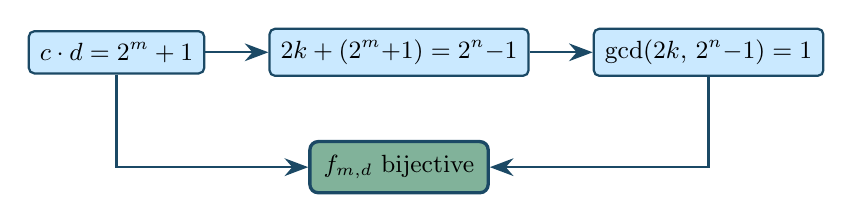
\begin{tikzpicture}[node distance=8mm,every node/.style={font=\small}]
  \node[box](i1){$c\cdot d=2^{m}+1$};
  \node[box,right=of i1](i2){$2k+(2^{m}{+}1)=2^{n}{-}1$};
  \node[box,right=of i2](i3){$\gcd(2k,\,2^{n}{-}1)=1$};
  \draw[maparrow](i1)--(i2);\draw[maparrow](i2)--(i3);
  \node[chip,fill=cE,below=8mm of i2](o){$f_{m,d}$ bijective};
  \draw[maparrow](i3) |- (o);\draw[maparrow](i1)|-(o);
\end{tikzpicture}
\end{center}

\vspace{3mm}
\heading{one map, two names}{Dempwolff--Müller polynomial $\ \equiv\ $ Cohen--Matthews polynomial}

\begin{center}
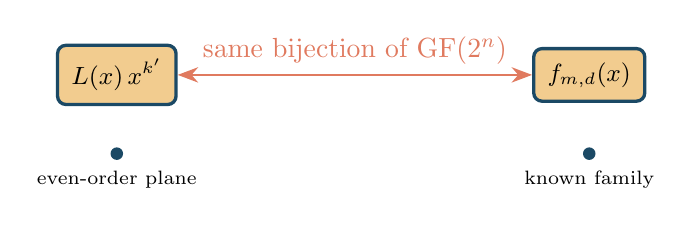
\begin{tikzpicture}[scale=1]
  \node[chip] (l) at (-3,0){$L(x)\,x^{k'}$};
  \node[chip] (r) at (3,0){$f_{m,d}(x)$};
  \draw[bij] (l)--(r) node[midway,above]{same bijection of $\GF{2^{n}}$};
  \node[dot] at (-3,-1){};\node[dot] at (3,-1){};
  \node[below] at (-3,-1.1){\scriptsize even-order plane};
  \node[below] at (3,-1.1){\scriptsize known family};
\end{tikzpicture}
\end{center}

\newpage
% =============================================================
% 7. Subfield trace tower
% =============================================================
\heading{7. Subfield traces --- a tower}{$\Tr_{n:d}$ folds $\GF{2^n}$ down onto $\GF{2^d}$}

\begin{center}
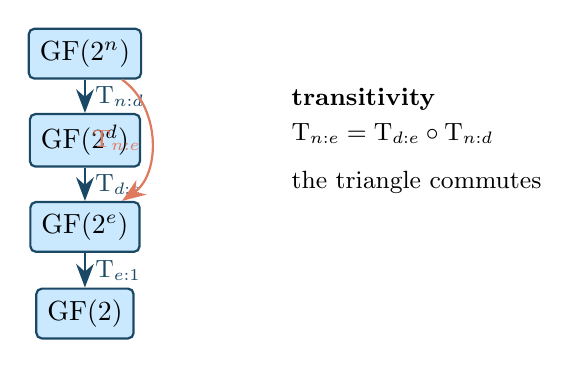
\begin{tikzpicture}[scale=1.1]
  % subgroup lattice / tower e | d | n
  \node[box] (n) at (0,3) {$\GF{2^{n}}$};
  \node[box] (d) at (0,2) {$\GF{2^{d}}$};
  \node[box] (e) at (0,1) {$\GF{2^{e}}$};
  \node[box] (o) at (0,0) {$\GF{2}$};
  \draw[maparrow] (n)--(d) node[midway,right,font=\small]{$\Tr_{n:d}$};
  \draw[maparrow] (d)--(e) node[midway,right,font=\small]{$\Tr_{d:e}$};
  \draw[maparrow] (e)--(o) node[midway,right,font=\small]{$\Tr_{e:1}$};
  \draw[maparrow,cD,bend left=55] (n) to node[left,font=\small]{$\Tr_{n:e}$} (e);
  \node[right=25mm,align=left,font=\small] at (0,2)
    {\textbf{transitivity}\\[2pt]$\Tr_{n:e}=\Tr_{d:e}\circ\Tr_{n:d}$\\[6pt]
     the triangle commutes};
\end{tikzpicture}
\end{center}

\vspace{1mm}
\heading{$\Tr_{n:d}$ = sum along a Frobenius orbit}{$x+x^{2^{d}}+x^{2^{2d}}+\dots$}

\begin{center}
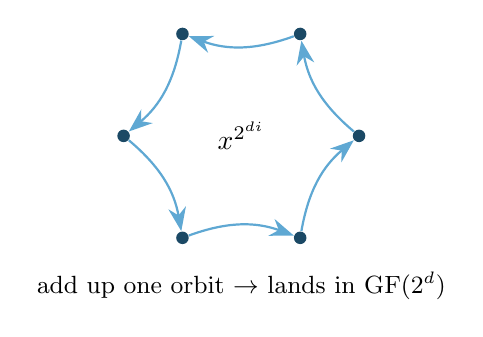
\begin{tikzpicture}[scale=1.15]
  \def\N{6}
  \foreach \i in {0,...,5}{\node[dot](o\i) at ({60*\i}:1.3){};}
  \foreach \i in {0,...,5}{\pgfmathtruncatemacro\j{Mod(\i+1,6)}
     \draw[maparrow,cB] (o\i) to[bend left=20] (o\j);}
  \node at (0,0){$x^{2^{di}}$};
  \node[below=1.6cm] at (0,0){\small add up one orbit $\to$ lands in $\GF{2^{d}}$};
\end{tikzpicture}
\end{center}

\vspace{1mm}
\heading{Lemma 4.11 --- $\widehat\Tr$ commutes with scaling}{$b\in\GF{2^{d}}$ slides through the hatted trace}

\begin{center}
\begin{tikzcd}[column sep=huge,row sep=large]
x \arrow[r,"\widehat\Tr_{n:e}"] \arrow[d,"b\cdot(-)"'] &
   \widehat\Tr_{n:e}x \arrow[d,"b\cdot(-)"]\\
b\,x \arrow[r,"\widehat\Tr_{n:d}"'] & b\cdot\widehat\Tr_{n:d}x
\end{tikzcd}
\end{center}

\newpage
% =============================================================
% 8. Semilinear operators & Singer group
% =============================================================
\heading{8. Semilinear operators $\Tr_r(a)$}{$x\mapsto a\,x^{2^{r}}$ --- twist by Frobenius, then scale}

\begin{center}
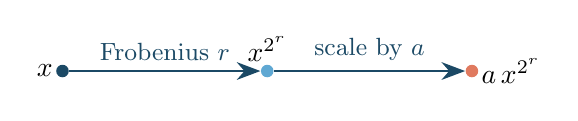
\begin{tikzpicture}[scale=1]
  \node[dot](x) at (0,0){};\node[left]at(x){$x$};
  \node[dot,fill=cB](f) at (2.6,0){};\node[above]at(f){$x^{2^{r}}$};
  \node[dot,fill=cD](y) at (5.2,0){};\node[right]at(y){$a\,x^{2^{r}}$};
  \draw[maparrow] (x)--(f) node[midway,above,font=\small]{Frobenius $r$};
  \draw[maparrow] (f)--(y) node[midway,above,font=\small]{scale by $a$};
\end{tikzpicture}
\end{center}

\vspace{2mm}
\heading{composition law}{$\Tr_r(a)\circ\Tr_s(b)=\Tr_{r+s}\!\big(a\,b^{2^{r}}\big)$}

\begin{center}
\begin{tikzcd}[column sep=large,row sep=large]
F \arrow[r,"\Tr_s(b)"] \arrow[dr,"\Tr_{r+s}(a\,b^{2^{r}})"'] & F \arrow[d,"\Tr_r(a)"]\\
 & F
\end{tikzcd}
\end{center}

\vspace{2mm}
\heading{Singer group = one big cycle}{$\Tr_0(a):x\mapsto ax$ acts sharply transitively on $F^\ast$}

\begin{center}
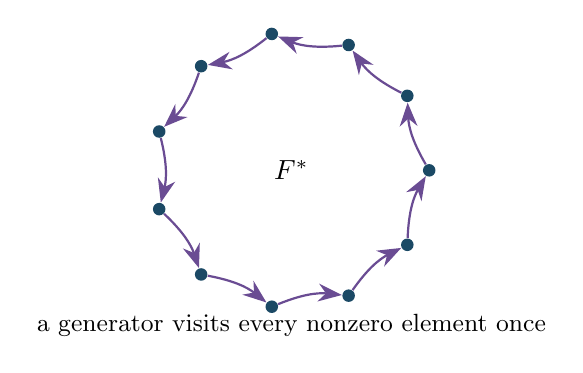
\begin{tikzpicture}[scale=1.25]
  \def\N{11}
  \foreach \i in {1,...,\N}{\node[dot](s\i) at ({360/\N*\i}:1.4){};}
  \foreach \i in {1,...,\N}{\pgfmathtruncatemacro\j{Mod(\i,\N)+1}
     \draw[maparrow,cG] (s\i) to[bend left=14] (s\j);}
  \node at (0,0){$F^\ast$};
  \node[below=1.7cm] at (0,0){\small a generator visits every nonzero element once};
\end{tikzpicture}
\end{center}

\newpage
% =============================================================
% 9. Lemma 4.2 support shift
% =============================================================
\heading{9. Lemma 4.2 --- conjugation shifts the support}{$\mathrm{spi}\big(\Tr_s(a)\,L\,\Tr_t(b)^{-1}\big)=\{\,i+r\bmod n\,\}$, \ $r=s-t$}

\begin{center}
\begin{tikzpicture}[scale=1.2]
  % ring of n slots, filled = in support
  \def\N{8}
  \foreach \i in {0,...,7}{
    \node[odot] (c\i) at ({45*\i}:1.5){};
    \node[font=\scriptsize] at ({45*\i}:1.9){\i};
  }
  \foreach \i in {1,3,6}{\node[dot,fill=cD] at ({45*\i}:1.5){};}
  \node at (0,0){$\mathrm{spi}(L)$};
\end{tikzpicture}
\qquad\Large$\xrightarrow{\ +r\ }$\qquad
\begin{tikzpicture}[scale=1.2]
  \def\N{8}
  \foreach \i in {0,...,7}{
    \node[odot] (c\i) at ({45*\i}:1.5){};
    \node[font=\scriptsize] at ({45*\i}:1.9){\i};
  }
  \foreach \i in {3,5,0}{\node[dot,fill=cE] at ({45*\i}:1.5){};}
  \node at (0,0){shifted};
\end{tikzpicture}
\end{center}

\begin{center}\small
support beads rotate rigidly by $r$ around $\mathbb Z/n$ --- pattern preserved.
\end{center}

\vspace{3mm}
\heading{additive polynomial = beads on a necklace}{$L(x)=\sum_i a_i x^{2^{i}}$; support $=$ which beads are lit}

\begin{center}
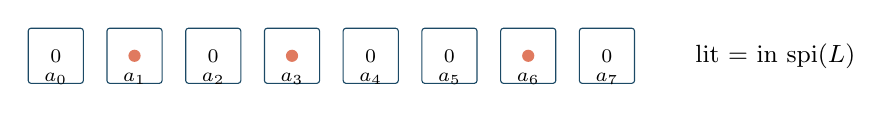
\begin{tikzpicture}[scale=1]
  \foreach \i in {0,...,7}{
     \node[draw=cA,minimum size=7mm,rounded corners=1pt] (b\i) at (\i,0){};
     \node[below=1mm] at (b\i){\scriptsize $a_{\i}$};
  }
  \foreach \i in {1,3,6}{\fill[cD] (b\i.center) circle(2.2pt);}
  \foreach \i in {0,2,4,5,7}{\node at (b\i.center){\scriptsize$0$};}
  \node[right=4mm,font=\small] at (7.6,0){lit $=$ in $\mathrm{spi}(L)$};
\end{tikzpicture}
\end{center}

\newpage
% =============================================================
% 10. Lemma 6.1(a) symplectic adjoint
% =============================================================
\heading{10. Lemma 6.1(a) --- symplectic adjoint}{under the trace form, $\Tr_k(b)^{\ast}=\Tr_{n-k}\!\big(b^{2^{\,n-k}}\big)$}

\begin{center}
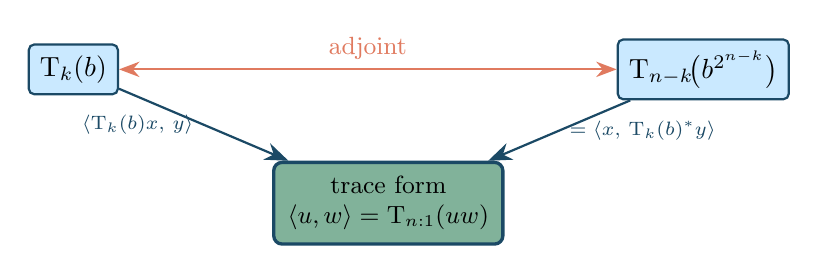
\begin{tikzpicture}[scale=1]
  \node[chip,fill=cE](form) at (0,0){trace form\\$\langle u,w\rangle=\Tr_{n:1}(uw)$};
  \node[box](op) at (-4,1.7){$\Tr_k(b)$};
  \node[box](adj) at (4,1.7){$\Tr_{n-k}\!\big(b^{2^{n-k}}\big)$};
  \draw[bij](op)--(adj) node[midway,above,font=\small]{adjoint};
  \draw[maparrow](op)--(form) node[midway,left,font=\scriptsize]{$\langle \Tr_k(b)x,\,y\rangle$};
  \draw[maparrow](adj)--(form) node[midway,right,font=\scriptsize]{$=\langle x,\,\Tr_k(b)^{\ast}y\rangle$};
\end{tikzpicture}
\end{center}

\vspace{2mm}
\heading{index reflection}{$k \leftrightarrow n-k$ mirrored around the circle}

\begin{center}
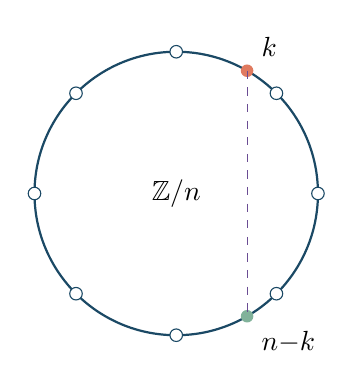
\begin{tikzpicture}[scale=1.2]
  \draw[cA,thick] (0,0) circle(1.5);
  \foreach \i in {0,...,7}{\node[odot] at ({45*\i}:1.5){};}
  \node[dot,fill=cD,label=above right:$k$] at (60:1.5){};
  \node[dot,fill=cE,label=below right:$n{-}k$] at (-60:1.5){};
  \draw[dashed,cG] (60:1.5)--(-60:1.5);
  \node at (0,0){$\mathbb Z/n$};
\end{tikzpicture}
\end{center}

\vspace{2mm}
\heading{self-adjoint spread = symplectic}{adjoint pairs the operators; the trace form is the glue}

\begin{center}
\begin{tikzcd}[column sep=huge,row sep=large]
F \arrow[r,"\Tr_k(b)"] \arrow[d,"{\langle\,,\rangle}"'] & F \arrow[d,"{\langle\,,\rangle}"]\\
F^{\vee} & F^{\vee} \arrow[l,"\Tr_{n-k}(b^{2^{n-k}})"]
\end{tikzcd}
\end{center}

\newpage
% =============================================================
% 11. Frobenius periodicity (FrobAlg)
% =============================================================
\heading{11. Frobenius --- a clock of period $n$}{$x\mapsto x^{2}$ cycles back after $n$ steps on $\GF{2^{n}}$}

\begin{center}
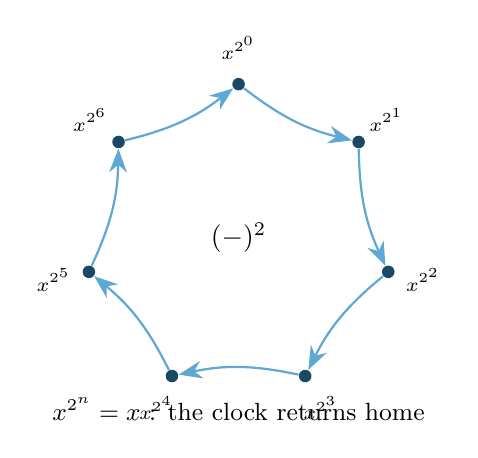
\begin{tikzpicture}[scale=1.3]
  \def\N{7}
  \foreach \i in {0,...,6}{
    \node[dot] (t\i) at ({90-360/\N*\i}:1.5){};
    \node[font=\scriptsize] at ({90-360/\N*\i}:1.85){$x^{2^{\i}}$};
  }
  \foreach \i in {0,...,6}{\pgfmathtruncatemacro\j{Mod(\i+1,\N)}
     \draw[maparrow,cB] (t\i) to[bend right=12] (t\j);}
  \node at (0,0){$(-)^{2}$};
  \node[below=1.9cm] at (0,0){\small $x^{2^{n}}=x$ : the clock returns home};
\end{tikzpicture}
\end{center}

\vspace{2mm}
\heading{linearized polynomials ride the clock}{Frobenius is additive: powers of $2$ pass through sums}

\begin{center}
\begin{tikzcd}[column sep=huge,row sep=large]
(x{+}y) \arrow[r,"(-)^{2^{j}}"] \arrow[d,equal] & (x{+}y)^{2^{j}} \arrow[d,equal]\\
x{+}y \arrow[r,"(-)^{2^{j}}"'] & x^{2^{j}}{+}y^{2^{j}}
\end{tikzcd}
\end{center}

\vspace{4mm}
% ---- closing legend ----
\heading{Legend of pictures}{how to read the shapes}

\begin{center}
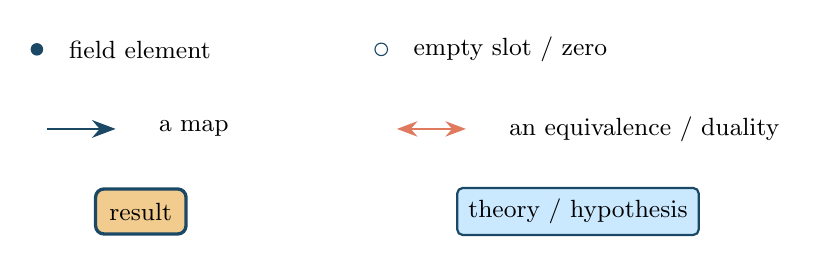
\begin{tikzpicture}[node distance=3mm,every node/.style={font=\small}]
  \node[dot](d){}; \node[right=2mm of d]{field element};
  \node[odot,right=42mm of d](o){}; \node[right=2mm of o]{empty slot / zero};
  \node[below=8mm of d](a1){}; \draw[maparrow] (a1)--++(1,0);
     \node[right=13mm of a1]{a map};
  \node[right=42mm of a1](a2){}; \draw[bij](a2)--++(1,0);
     \node[right=13mm of a2]{an equivalence / duality};
  \node[below=8mm of a1](c1){}; \node[chip,right=6mm of c1]{result};
  \node[box,right=52mm of c1]{theory / hypothesis};
\end{tikzpicture}
\end{center}

\vfill
\begin{center}\footnotesize
Each diagram is a faithful picture of a statement proved in the Lean library
(\texttt{RequestProject/DempwolffMueller/}). No claim here is stronger than its
machine-checked counterpart.
\end{center}

\end{document}
